\documentclass{beamer}

\mode<presentation> {
\usetheme{Warsaw}
}
\usepackage{polski}
\usepackage{graphicx} % Allows including images
\usepackage{booktabs} % Allows the use of \toprule, \midrule and \bottomrule in tables


\title[NIDUC 2 - kody FEC]{NIDUC 2 - kody FEC}

\author{Kamil Bońkowski, Wiktor Porowski, Tomasz Rzymyszkiewicz} 
\institute[PWr] 
{
Politechnika Wrocławska \\ 
}
\date{czerwiec 2021}
\begin{document}

\begin{frame}
\titlepage
\end{frame}

\begin{frame}
\frametitle{Plan prezentacji}
\tableofcontents 
\end{frame}

\section{Testy zdolności korekcyjnych badanych kodów FEC} 

\subsection{Potrajanie bitów} 

\begin{frame}
\frametitle{AAABBBCCC}

Nadmiarowość = 0,66

\begin{figure}
    \centering
    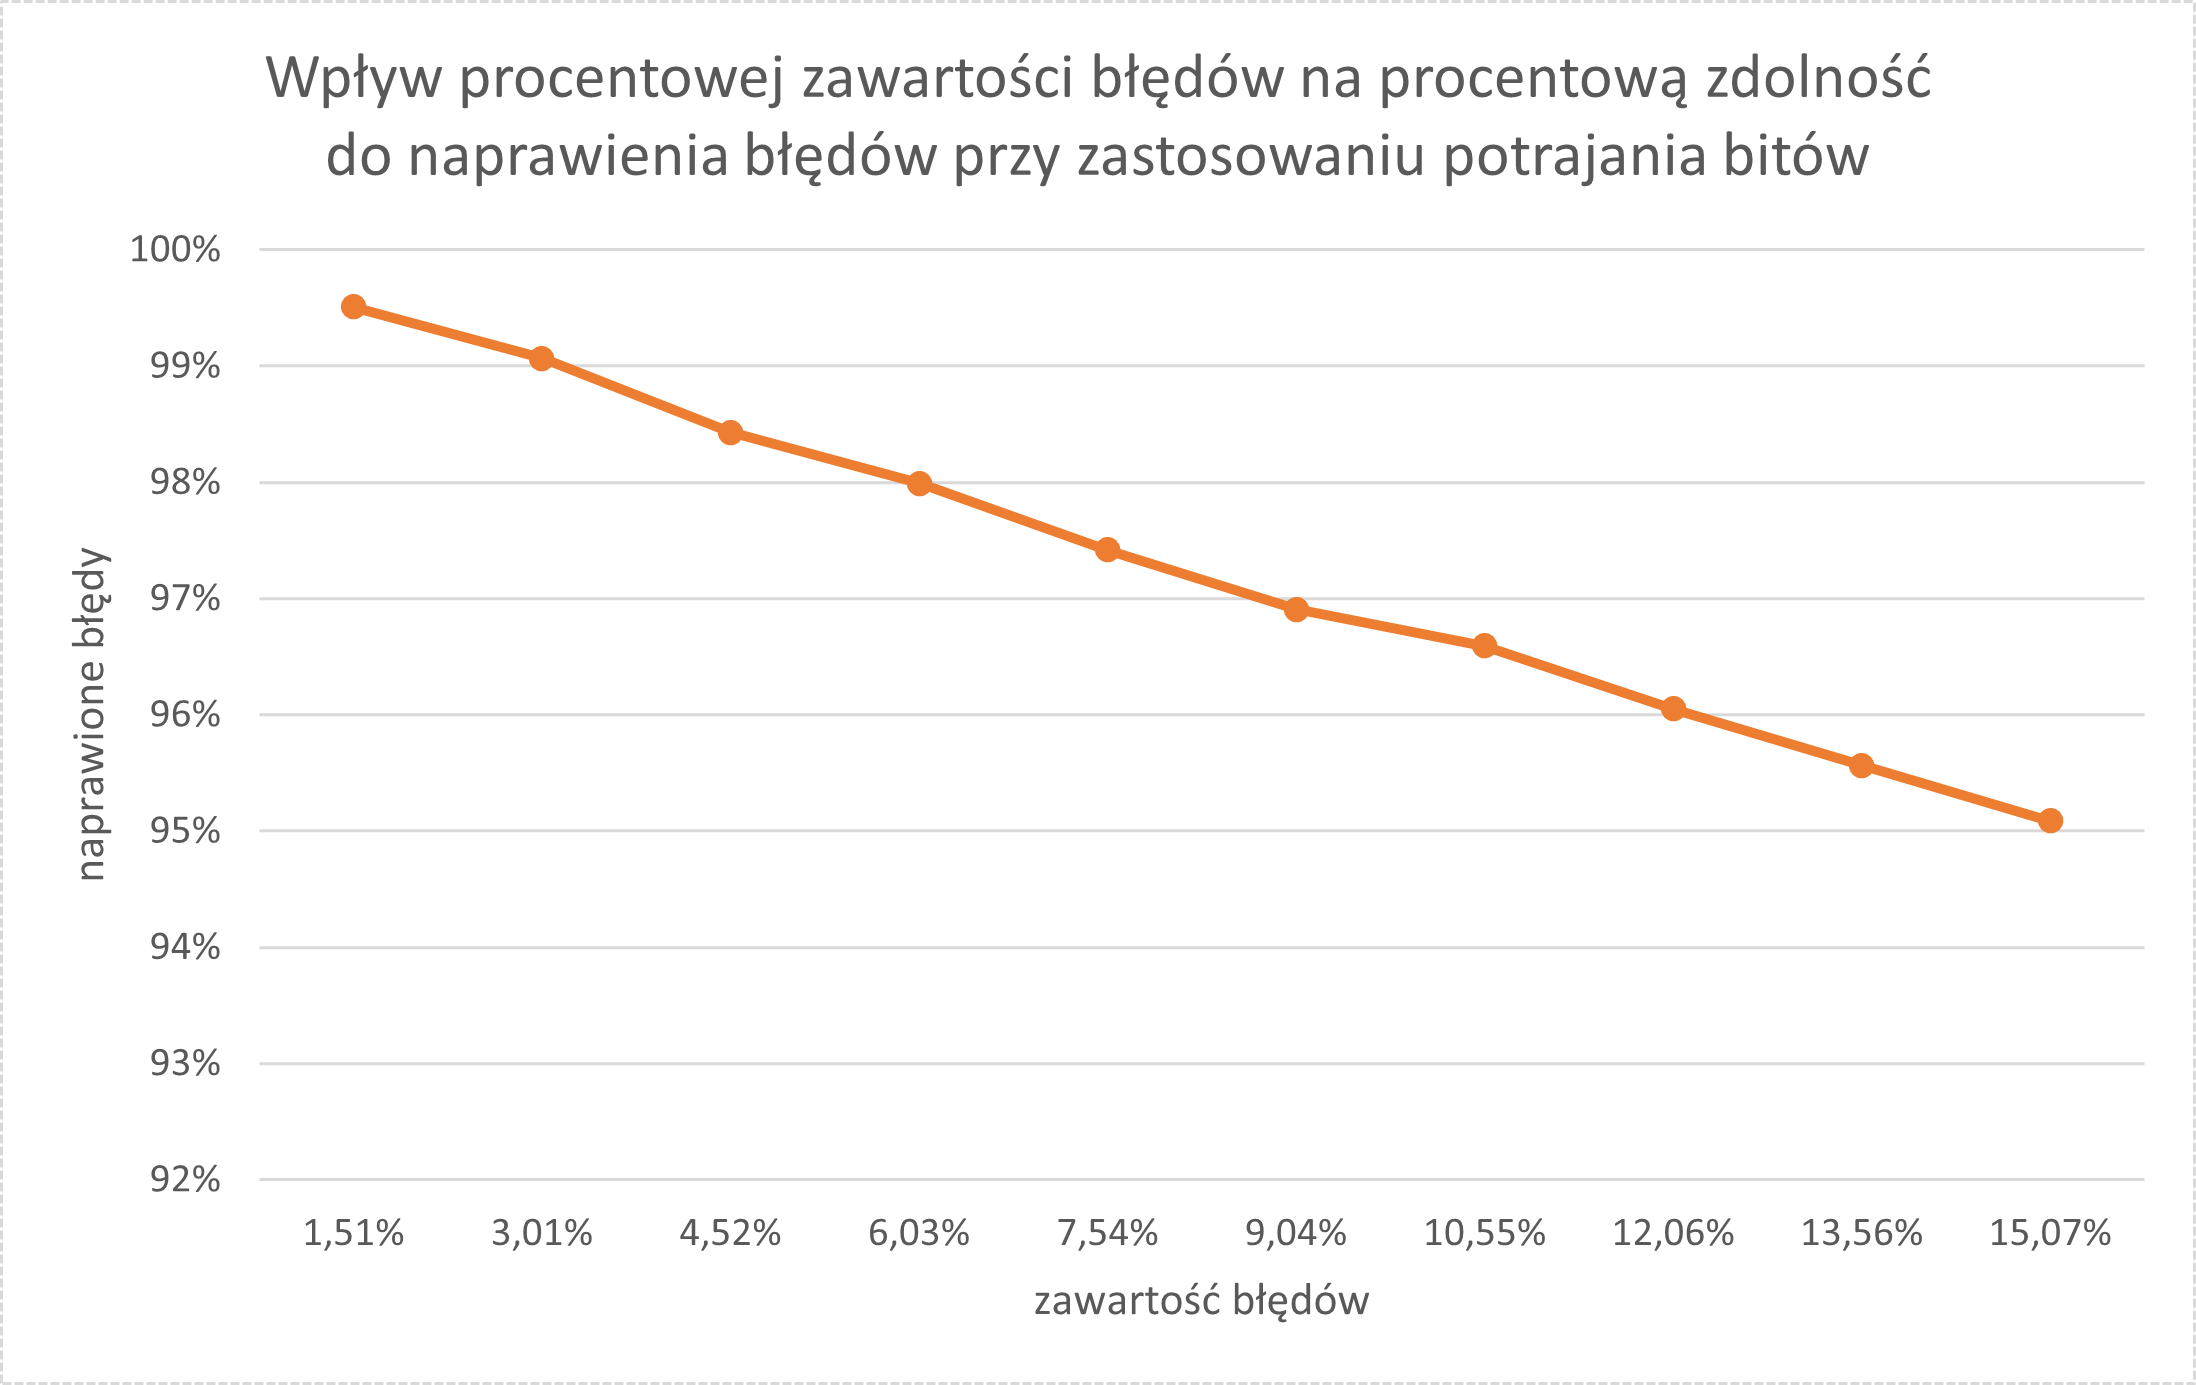
\includegraphics[scale=0.5]{wykresy/potrajanie_aaa.png}
\end{figure}
\end{frame}


\begin{frame}
\frametitle{ABCABCABC}

Nadmiarowość = 0,66

\begin{figure}
    \centering
    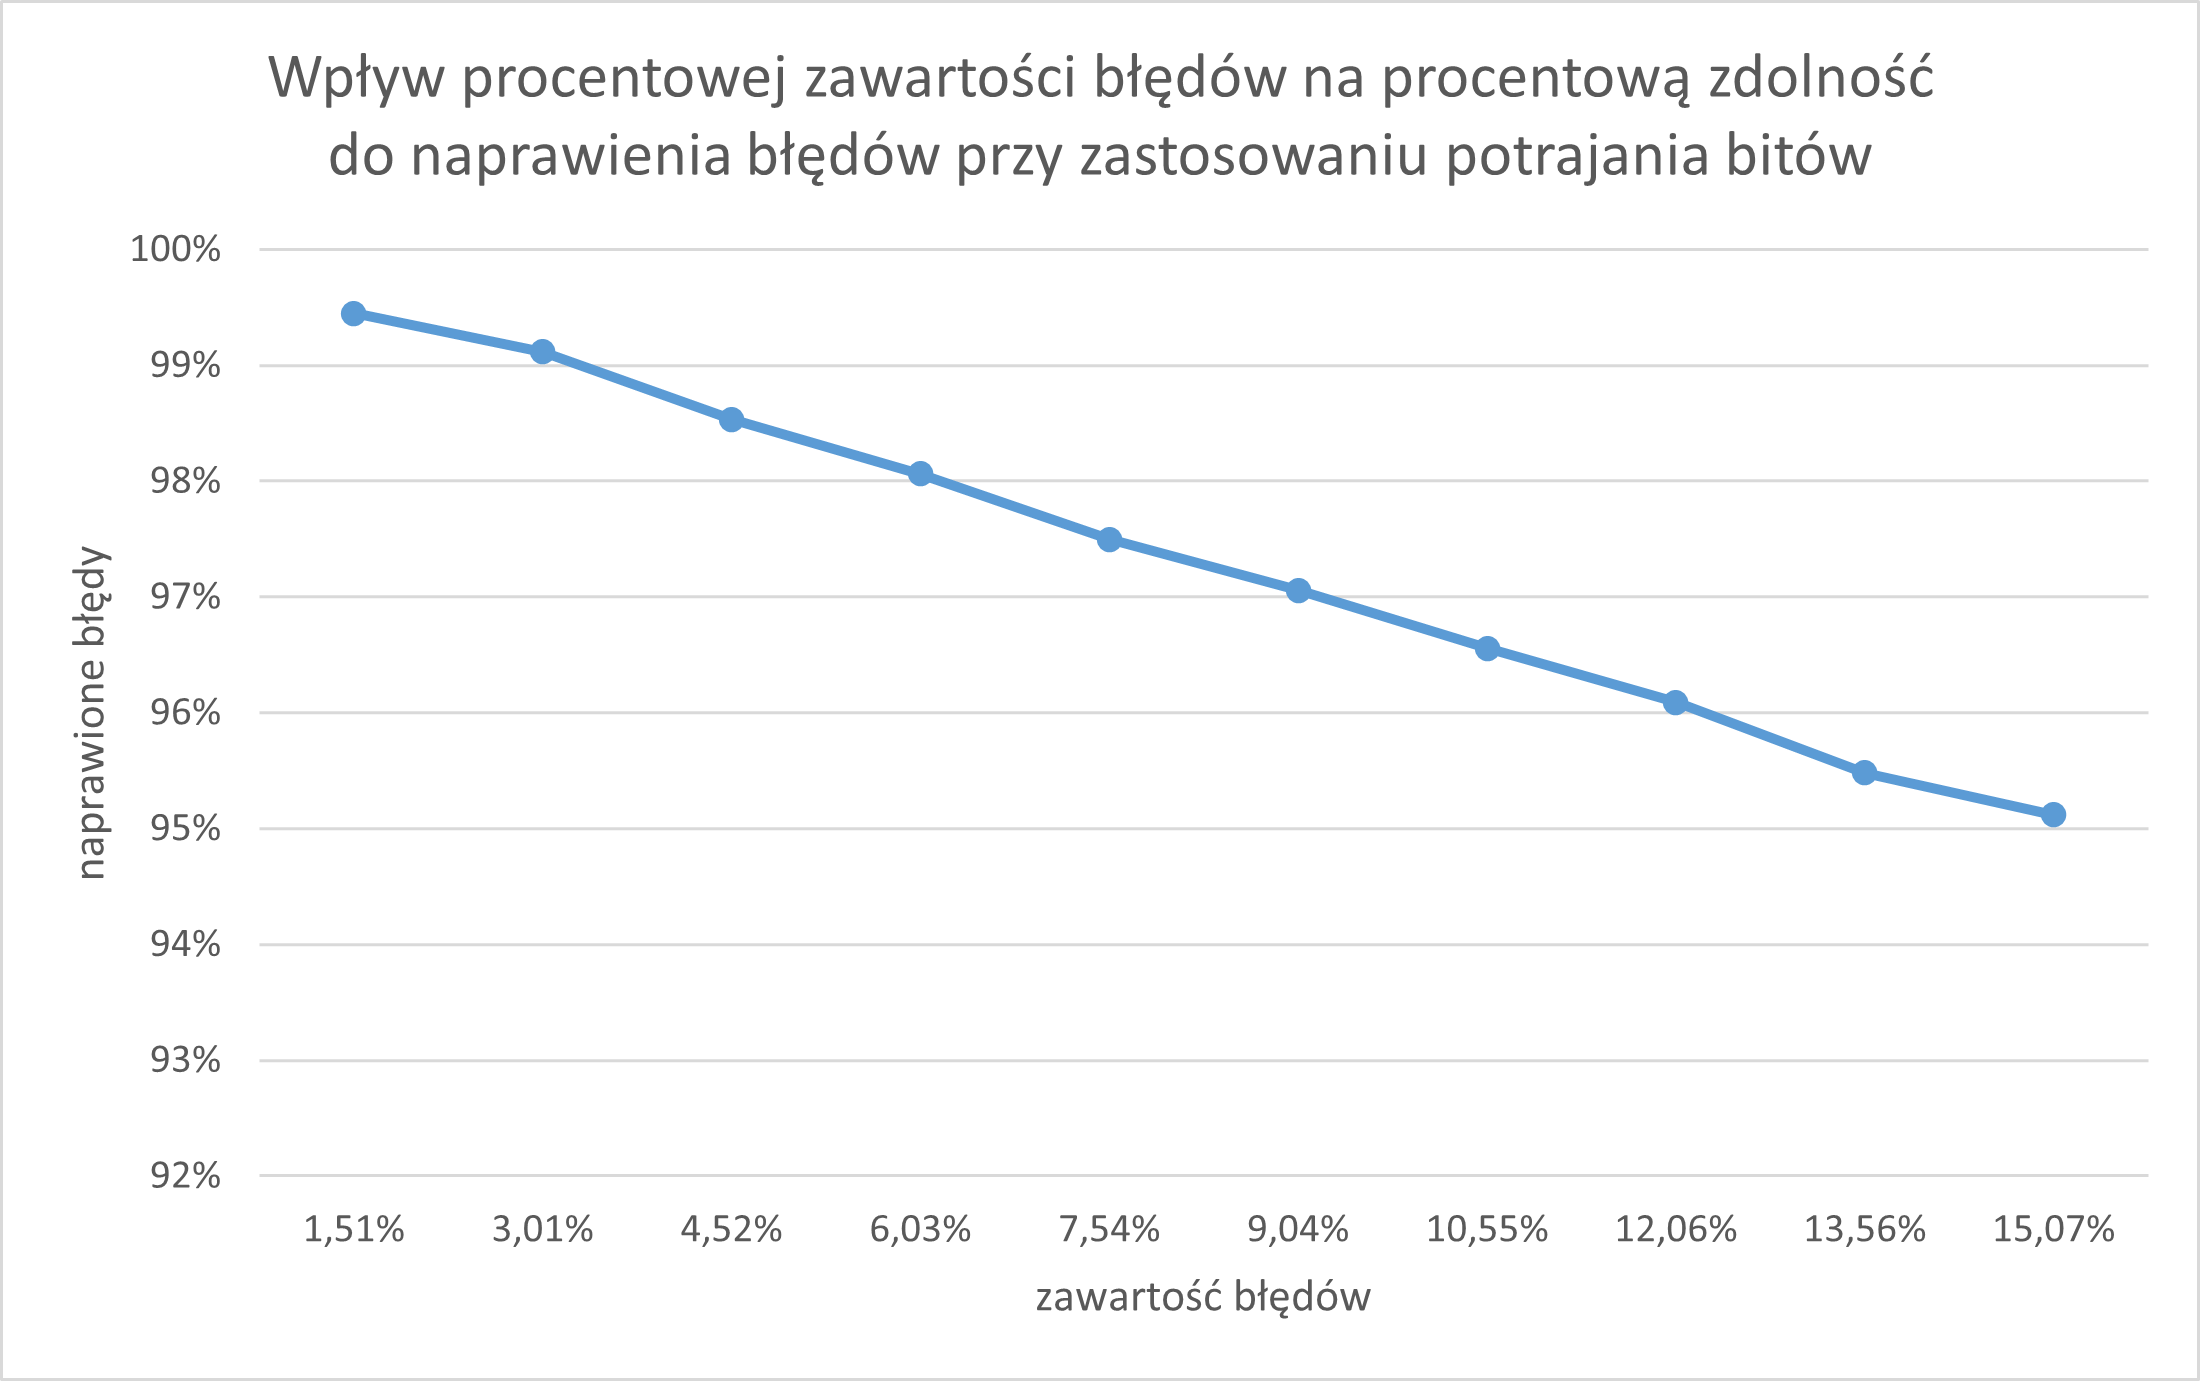
\includegraphics[scale=0.5]{wykresy/potrajanie_abc.png}
\end{figure}

\end{frame}

\subsection{Kod BCH}
\begin{frame}

Nadmiarowość = 0,49

\frametitle{BCH(5,3)}
\begin{figure}
    \centering
    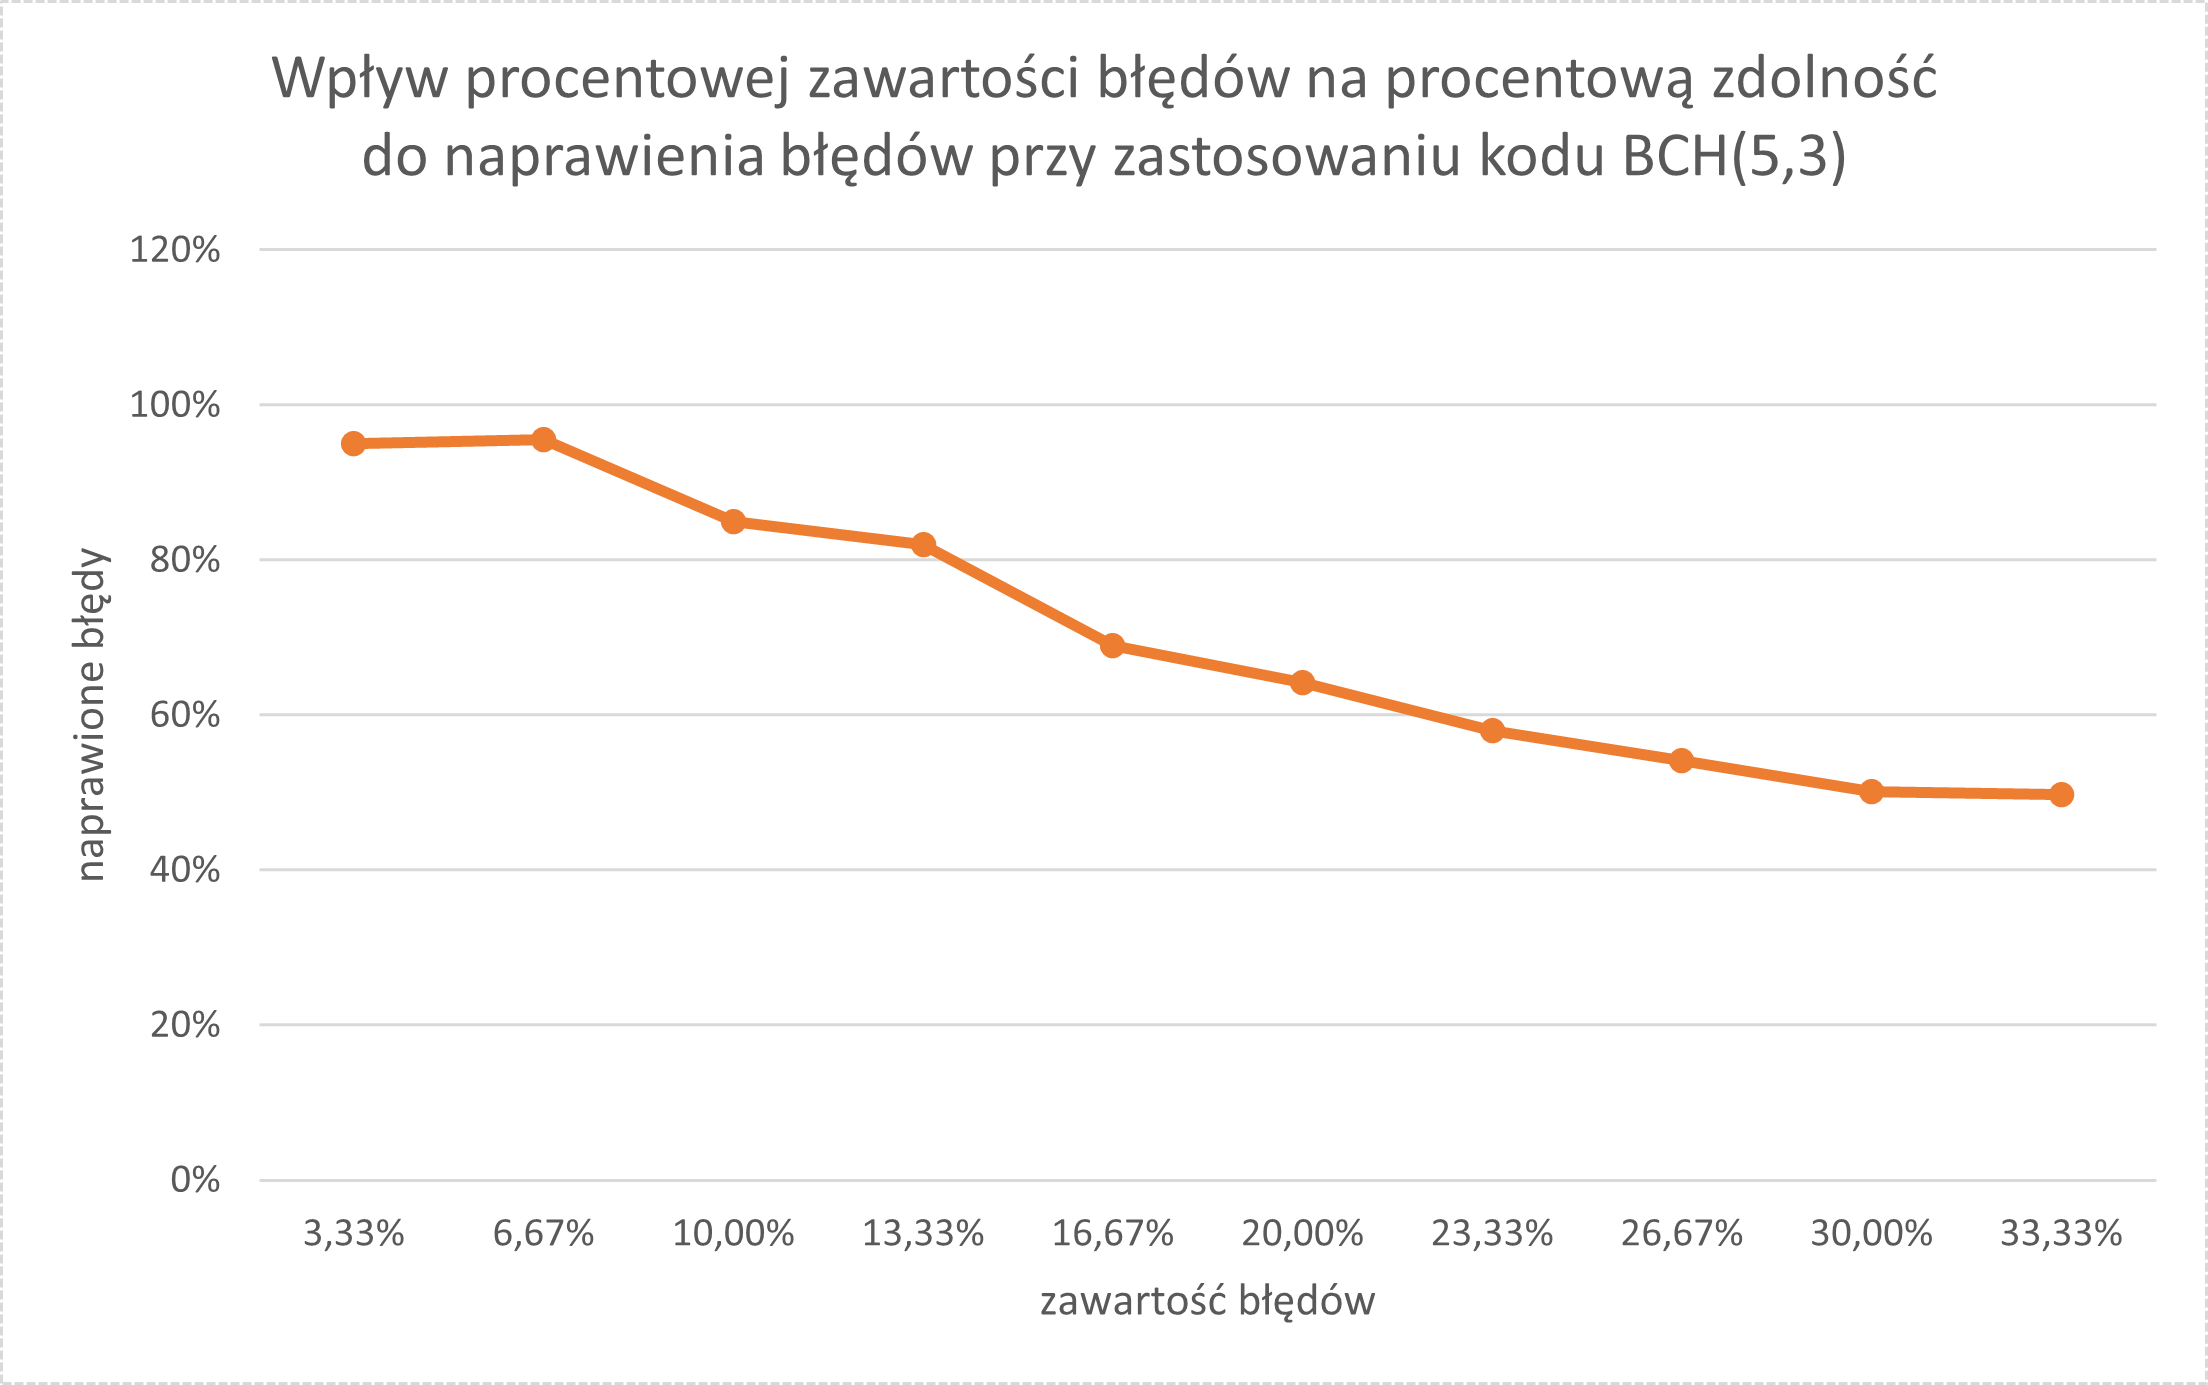
\includegraphics[scale=0.5]{wykresy/bch.png}
\end{figure}

\end{frame}

\subsection{Kody Hamminga}

\begin{frame}
\frametitle{Hamming}
\tiny
\centering
Nadmiarowości
\begin{table}[]
    \begin{tabular}{|l|l|l|l|l|l|}
    \hline
    (7,4) & (15,11) & (31,26) & (63,57) & (127,120) & (255,247) \\ \hline
    0,43  & 0,27    & 0,16    & 0,096   & 0,056     & 0,032     \\ \hline
    \end{tabular}
\end{table}
\begin{figure}
    \centering
    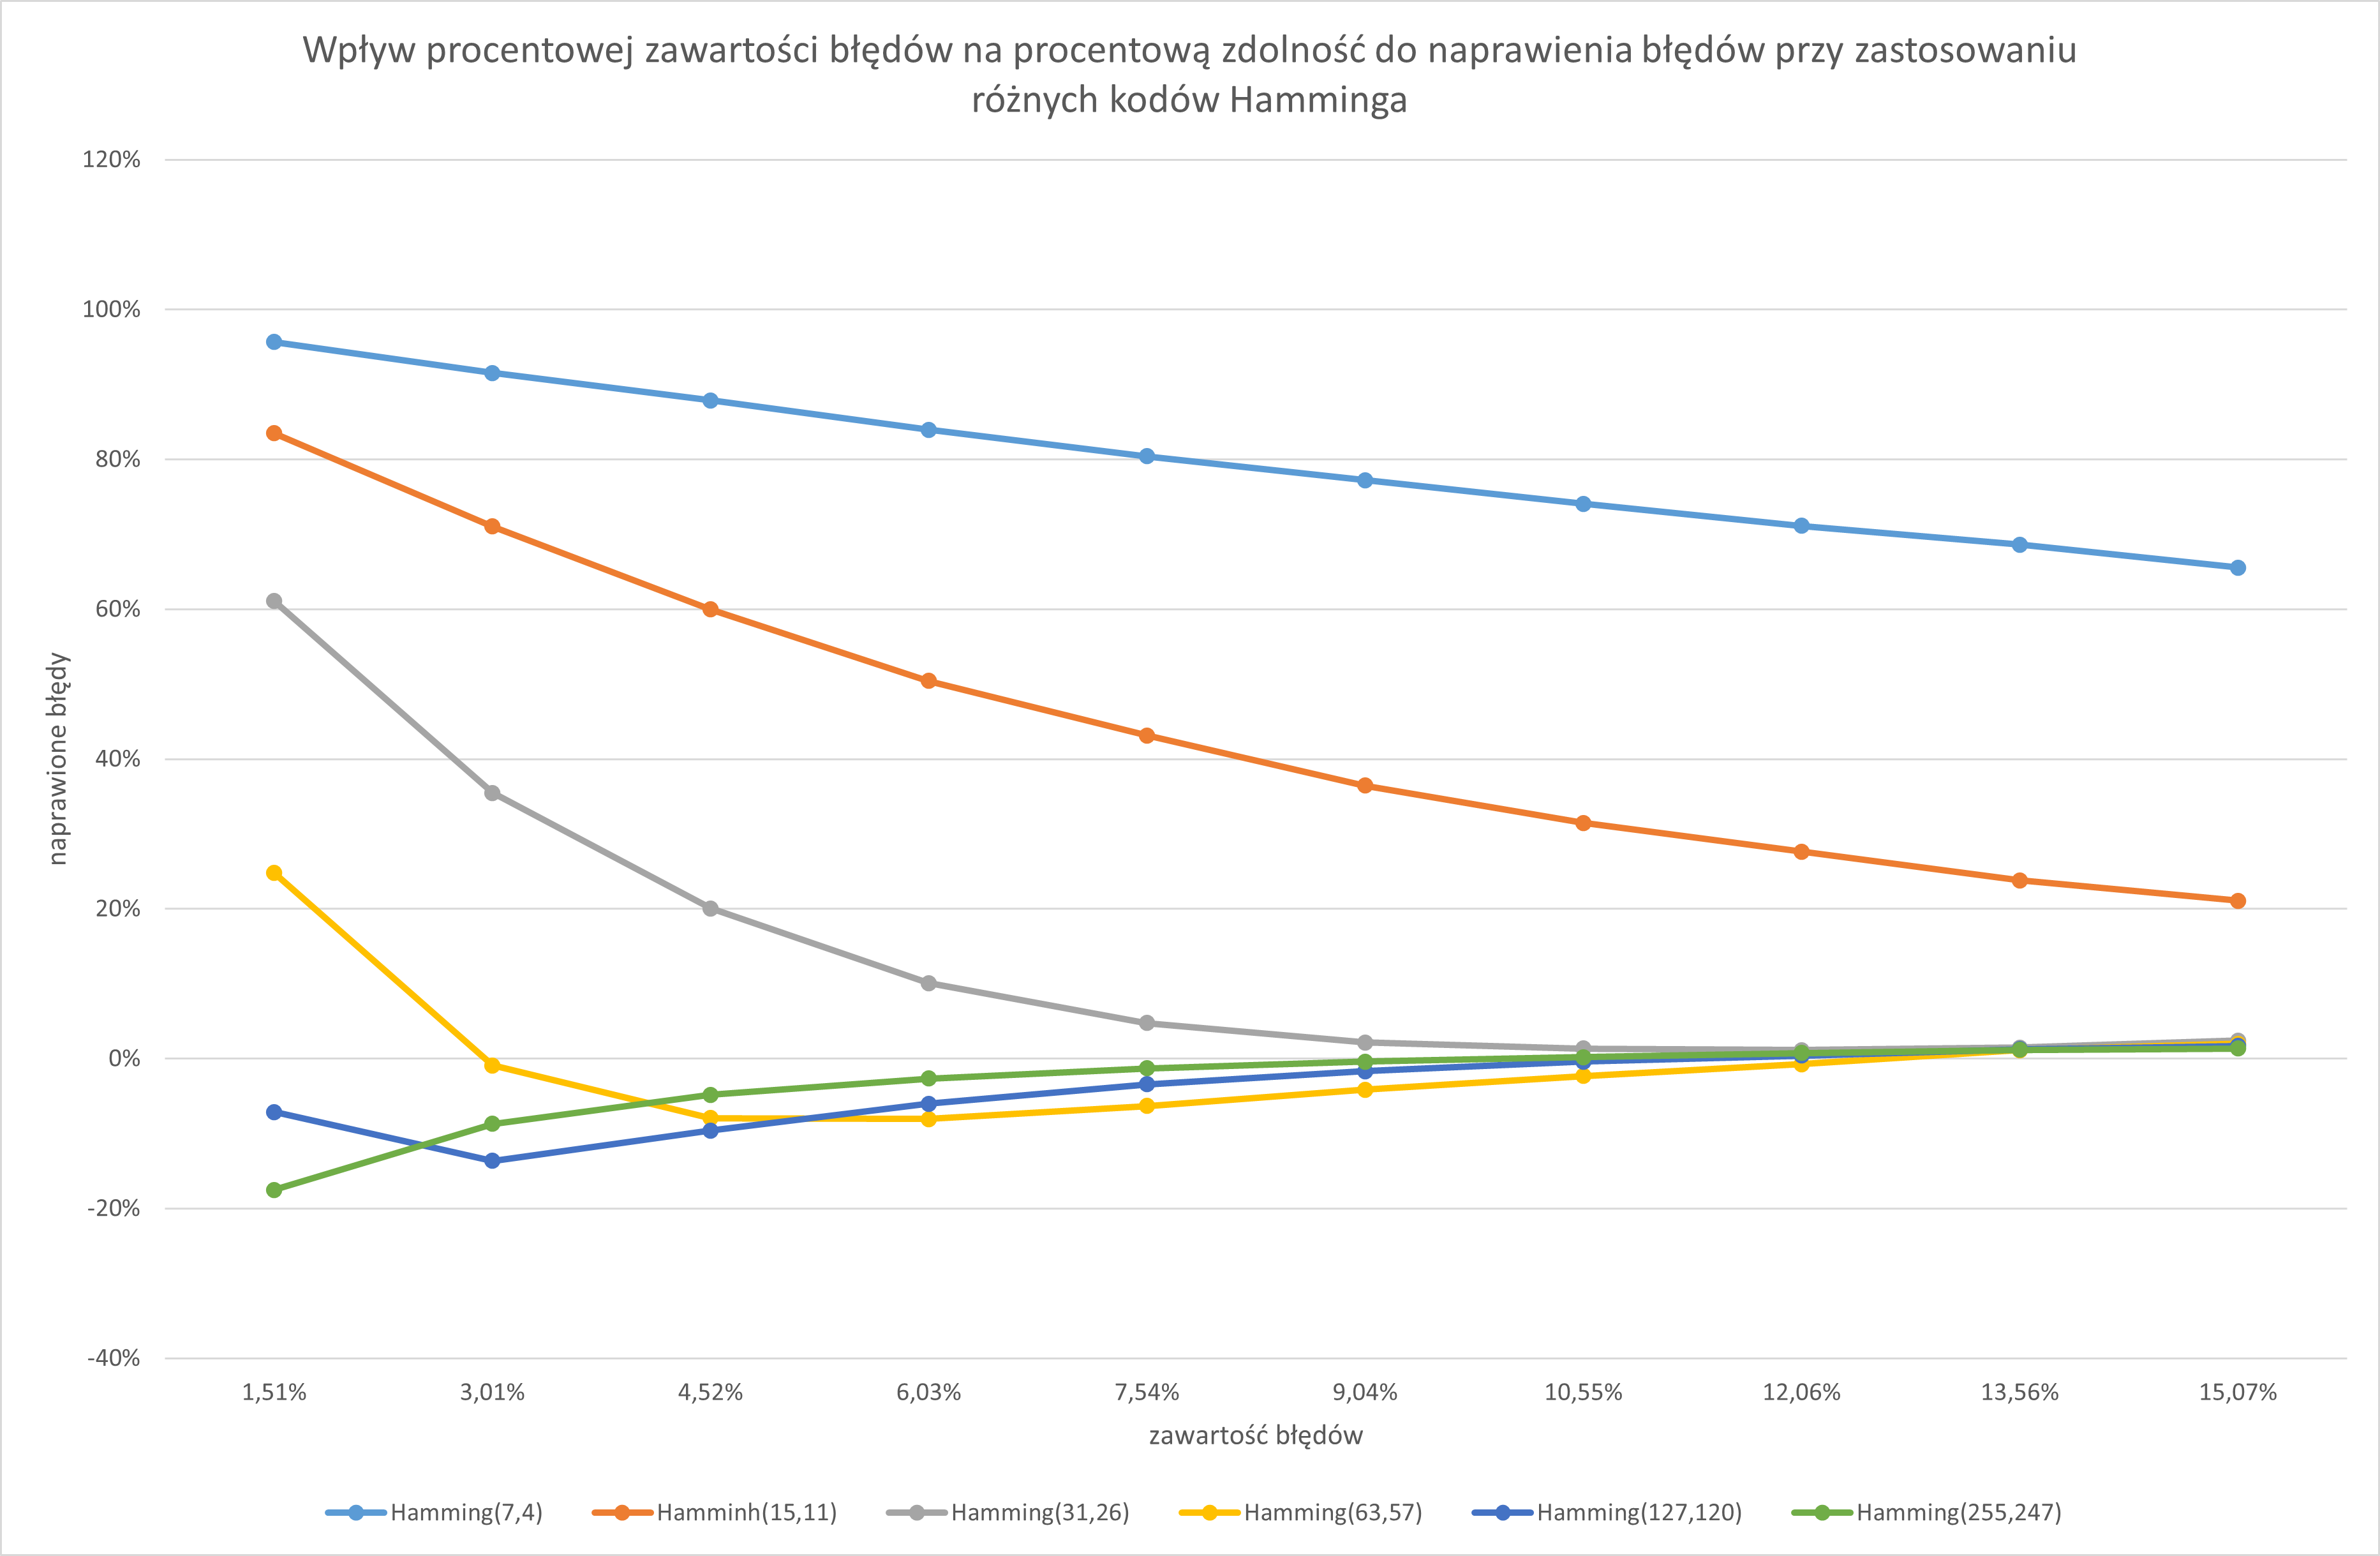
\includegraphics[scale=0.3]{wykresy/hamming.png}
\end{figure}
\end{frame}

\section{Zobrazowanie działania kodów na przykładzie grafiki}
\subsection{Oryginalna grafika testowa}
\begin{frame}
    \frametitle{Oryginalna grafika testowa}
    \begin{figure}
        \centering
        
\includegraphics[scale=4]{zdjecia/image.jpg}
    \end{figure}
\end{frame}


\subsection{Potrajanie bitów ABC}

\begin{frame}
\frametitle{Potrajanie bitów ABC}
\begin{columns}[c]
    \column{.5\textwidth}
    \tiny
    Grafika z błędami (100 tysięcy błędów) 
    \begin{figure}
        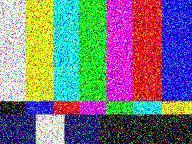
\includegraphics[scale=0.5]{zdjecia/grafika 100k bledow.jpg}
    \end{figure}
    
    \column{.5\textwidth}
    \tiny
    Grafika zakodowana i zdekodowana (100 tysięcy błędów)
    \begin{figure}
        
\includegraphics[scale=0.5]{zdjecia/grafika 100k bledow tripling.jpg}
    \end{figure}
\end{columns}
\end{frame}

\subsection{Kod Hamminga(7,4)}
\begin{frame}
\frametitle{Kod Hamminga(7,4)}
    \begin{columns}[c]
        \column{.5\textwidth}
        \tiny
        Grafika z błędami (100 tysięcy błędów) 
        \begin{figure}
            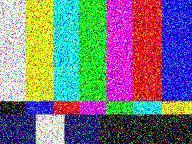
\includegraphics[scale=0.5]{zdjecia/grafika 100k bledow.jpg}
        \end{figure}
        
        \column{.5\textwidth}
        \tiny
        Grafika zakodowana i zdekodowana (100 tysięcy błędów)
        \begin{figure}
            
\includegraphics[scale=0.5]{zdjecia/grafika 100k bledow hamming.jpg}
        \end{figure}
    \end{columns}
\end{frame}

\section{Wnioski}

\begin{frame}
\frametitle{Wnioski}
\begin{itemize}
    \item wydajność potrajania bitów a zdolność korekcyjna
    \item błędy grupowe a kod Hamminga (BCH)
    \item ujemna zdolność korekcyjna w liczbie błędów zbliżonej do liczby bloków (kształt wykresu)
    \item porównanie kodów
\end{itemize}
\end{frame}

\end{document} 